\documentclass{beamer}
%
% Choose how your presentation looks.
%
% For more themes, color themes and font themes, see:
% http://deic.uab.es/~iblanes/beamer_gallery/index_by_theme.html
%
\mode<presentation>
{
  \usetheme{default}      % or try Darmstadt, Madrid, Warsaw, ...
  \usecolortheme{default} % or try albatross, beaver, crane, ...
  \usefonttheme{default}  % or try serif, structurebold, ...
  \setbeamertemplate{navigation symbols}{}
  \setbeamertemplate{caption}[numbered]
  \setbeamertemplate{footline}[frame number]
} 

\usepackage[english]{babel}
\usepackage[utf8x]{inputenc}
\usepackage{listings}
\usepackage{courier}

\title[2016-05-11-scala-spark]{Scala and Spark Tutorial}
\author{Jim Pivarski}
\institute{Princeton University -- DIANA}
\date{May 11, 2016}

\xdefinecolor{darkblue}{rgb}{0.1,0.1,0.7}
\definecolor{commentgreen}{rgb}{0,0.6,0}
\definecolor{stringmauve}{rgb}{0.58,0,0.82}

\lstset{ %
  backgroundcolor=\color{white},      % choose the background color
  basicstyle=\ttfamily\small,         % size of fonts used for the code
  breaklines=true,                    % automatic line breaking only at whitespace
  captionpos=b,                       % sets the caption-position to bottom
  commentstyle=\color{commentgreen},  % comment style
  escapeinside={\%*}{*)},             % if you want to add LaTeX within your code
  keywordstyle=\color{blue},          % keyword style
  stringstyle=\color{stringmauve},    % string literal style
  showstringspaces=false,
  showlines=true
}

\begin{document}

\begin{frame}
  \titlepage
\end{frame}

% Uncomment these lines for an automatically generated outline.
%\begin{frame}{Outline}
%  \tableofcontents
%\end{frame}

\begin{frame}{}
\begin{description}
\item[Spark:] a data analysis framework

(like ROOT, but with different strengths and weaknesses).

\vspace{0.5 cm}

\item[Scala:] Spark's native language, used as a command prompt

(the way that C++ is used for ROOT).
\end{description}
\end{frame}

\begin{frame}{Outline}
\begin{enumerate}
\item 5 minute talk on Scala
\item $\sim$half hour Scala exercises
\item 5 minute talk on Spark
\item $\sim$hour and a half Spark exercises in Scala
\end{enumerate}
\end{frame}

\begin{frame}{}
\begin{columns}
\column{1.1\linewidth}

\includegraphics[width=\linewidth]{languages1.pdf}
\end{columns}
\end{frame}

\begin{frame}{}
\begin{columns}
\column{1.1\linewidth}
\includegraphics[width=\linewidth]{languages2.pdf}
\end{columns}
\end{frame}

\begin{frame}{}
\begin{columns}
\column{1.1\linewidth}
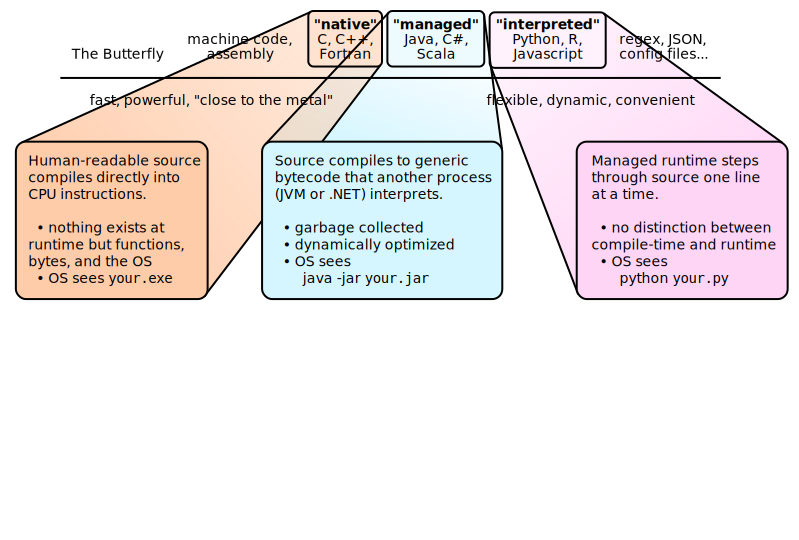
\includegraphics[width=\linewidth]{languages25.pdf}
\end{columns}
\end{frame}

\begin{frame}{}
\begin{center}
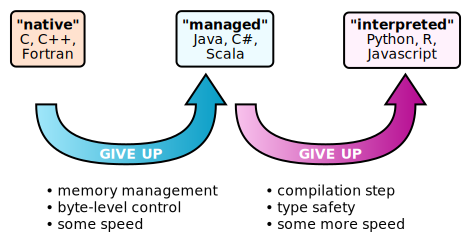
\includegraphics[width=0.8\linewidth]{languages3.pdf}
\end{center}
\end{frame}

\begin{frame}{}
\begin{center}
\includegraphics[width=0.8\linewidth]{languages4.pdf}
\end{center}
\end{frame}

\begin{frame}{What happens in the compilation step?}
\begin{itemize}
\item Whole program is interpreted and turned into machine instructions (possibly for a virtual machine).
\item All variables are interpreted as belonging to specific types: {\tt int}, {\tt string}, {\tt MissileController}\ldots
\item Uses of these variables are checked for validity:
\begin{itemize}
\item can't pass a {\tt MissileController} into the cosine function;
\item can't call {\tt launchAllMissiles()} on a {\tt string}.
\end{itemize}
\end{itemize}

\vfill
Interpreted languages do none of these things; you find out about misuses of variables at runtime (can be good, can be bad).
\end{frame}

\begin{frame}{Why should you care?}
\begin{itemize}
\item Compilation step can get in the way of testing a program one piece at a time.
\item The type check is a {\it formal proof} that the program is free of certain types of errors; it won't fail after hours of running.
\end{itemize}

\vfill
\begin{uncoverenv}<2->
\hspace{-0.83 cm} \textcolor{darkblue}{\Large Scala}

\begin{itemize}
\item Scala compiles to bytecode that runs on the Java Virtual Machine (JVM).
\item It emphasizes type safety (even more than C++).
\item It has extensive type inference to reduce annoyance,
\item and an interactive prompt for testing small components or interacting with a running program.
\end{itemize}
\end{uncoverenv}
\end{frame}

\begin{frame}{}
\begin{columns}
\column{1.18\linewidth}
\includegraphics[width=\linewidth]{jvm_languages.png}
\end{columns}
\end{frame}

\begin{frame}{}
\begin{columns}
\column{1.18\linewidth}
\includegraphics[width=\linewidth]{popularity1.png}
\end{columns}
\end{frame}

\begin{frame}{}
\begin{columns}
\column{1.18\linewidth}
\includegraphics[width=\linewidth]{popularity2.png}
\end{columns}
\end{frame}

\begin{frame}{}
\begin{center}
\Huge \textcolor{darkblue}{Scala Exercises}
\end{center}
\end{frame}

\end{document}
